\documentclass[compress,t]{beamer}
\newcommand{\thou}{,\!000}
% Copyright 2004 by Till Tantau <tantau@users.sourceforge.net>.
%
% In principle, this file can be redistributed and/or modified under
% the terms of the GNU Public License, version 2.
%
% However, this file is supposed to be a template to be modified
% for your own needs. For this reason, if you use this file as a
% template and not specifically distribute it as part of a another
% package/program, I grant the extra permission to freely copy and
% modify this file as you see fit and even to delete this copyright
% notice. 

\mode<presentation> {
  \usetheme{Malmoe}
  \usecolortheme{beaver}
  \setbeamercovered{transparent}
  \setbeamertemplate{navigation symbols}{{\small\insertpagenumber}}
%{{\normalsize\insertframenumber}}
  \setbeamertemplate{footline}{%
    \leavevmode%
    \hbox{\begin{beamercolorbox}[wd=\paperwidth,ht=0.5ex,dp=1.125ex,leftskip=.3cm,rightskip=.3cm plus1fil]{title in head/foot}%
    \end{beamercolorbox}}%
    \vskip0pt%
  }
  \setbeamertemplate{headline}{% %split theme}
  \leavevmode%
    \begin{beamercolorbox}[wd=.3\paperwidth,ht=2.5ex,dp=1.125ex]{section in head/foot}%
      \insertsectionnavigationhorizontal{.3\paperwidth}{\hskip0pt plus1filll}{}%
  \end{beamercolorbox}%
  \begin{beamercolorbox}[wd=.7\paperwidth,ht=2.5ex,dp=1.125ex]{subsection in head/foot}%
    \insertsubsectionnavigationhorizontal{.7\paperwidth}{}{\hskip0pt plus1filll}%
  \end{beamercolorbox}%
  }
  %\setbeamersize{sidebar width right=2ex}
  %{\usebeamercolor{sidebar}}
  %\setbeamertemplate{sidebar canvas right}{f \insertframenumber}
  %\insertpagenumber
}

\usepackage[english]{babel}
\usepackage[latin1]{inputenc}
\usepackage{helvet}
\usepackage{xspace}
% Or whatever. Note that the encoding and the font should match. If T1
% does not look nice, try deleting the line with the fontenc.
%\usepackage[T1]{fontenc}
\usepackage[normalem]{ulem}
\usepackage{calc}
\usepackage{verbatim}
\usepackage{multirow}
\usepackage{dcolumn}
\usepackage{multimedia} 
%\usepackage{amsbsy}
\usepackage{amsmath}

\newcommand{\arxiv}[1]{\href{http://arxiv.org/abs/#1}{arXiv:#1}}
\newcommand{\etal}{\textit{et al.~}}
\newcommand{\snr}[1]{\mathbb{SN}(#1)}

%\graphicspath{{figs-slides/}{figs-techreport/}}

\newcommand{\eg}{\emph{eg}}

% commands to add more space in \itemize environments
\newcommand{\bitmorespace}{%
  \addtolength{\itemsep}{0.5ex}%
  %\addtolength{\parskip}{0.5ex}%
  %\addtolength{\parsep}{0.5ex}%
  %\addtolength{\topsep}{0.5ex}%
  \vspace{0.5ex}%
}
\newcommand{\morespace}{\addtolength{\itemsep}{1ex}}
\newcommand{\Morespace}{\addtolength{\itemsep}{1.5ex}}


\newcommand{\commentout}[1]{}


\usefonttheme[onlymath]{serif}
\usepackage{multimedia} 
\usepackage{amsmath}
\graphicspath{{figs/}}

\title{Unsupervised learning \& Mixture models}
\author{Dustin Lang \\ {\small McWilliams Postdoc Fellow \\ Carnegie Mellon University \\ \emph{visiting} University of Waterloo}}
\date{Local Group Astrostats \hspace*{0.5em}/\hspace*{0.5em} 2015-06-04}

\begin{document}

\begin{frame}
  \titlepage
\end{frame}

\section{Intro}

\begin{frame}{The Machine Learning Landscape}%[plain]
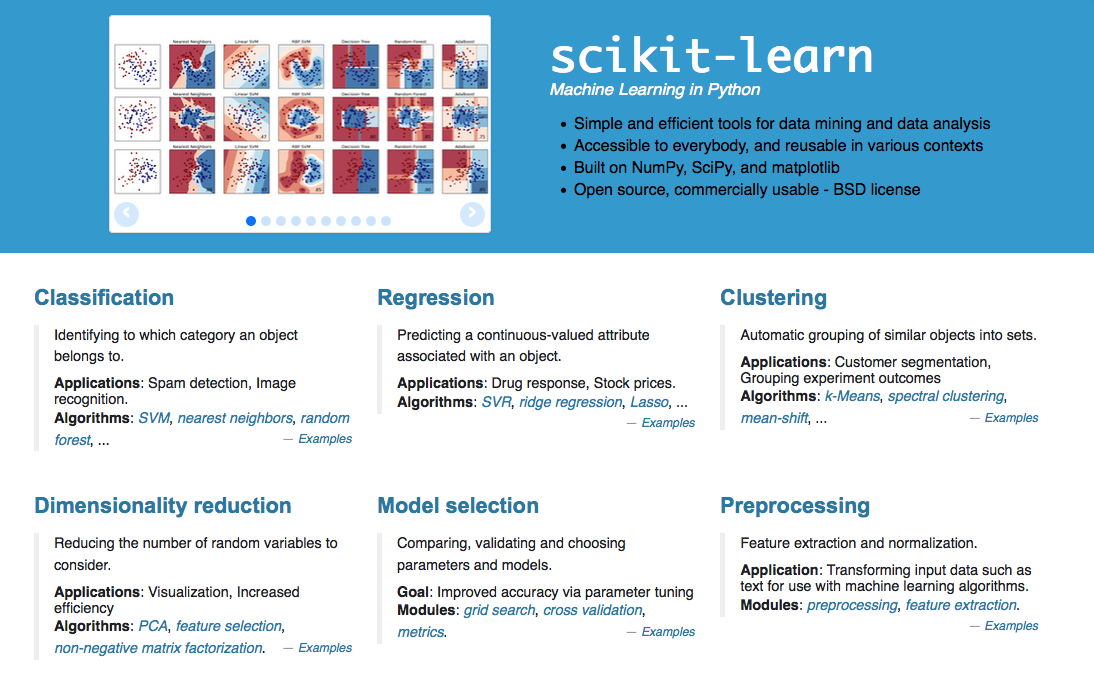
\includegraphics[width=\textwidth]{landscape}
\end{frame}

\begin{frame}{Unsupervised learning}
  \begin{itemize}
    \item \alert{No labels} / \alert{no truth}: We are not given a target value we want to reconstruct
    \item Just given the data (usually assumed: low-dimensional measurements
      with equal noise)
    \item Main task: \alert{Clustering}
  \end{itemize}

  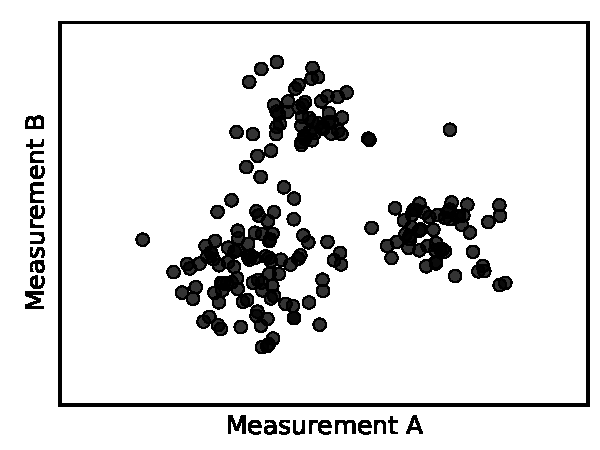
\includegraphics[width=0.4\textwidth]{ex3a}
  \hspace{1em}
  \raisebox{0.18\textheight}{$\longrightarrow$}
  \hspace{1em}
  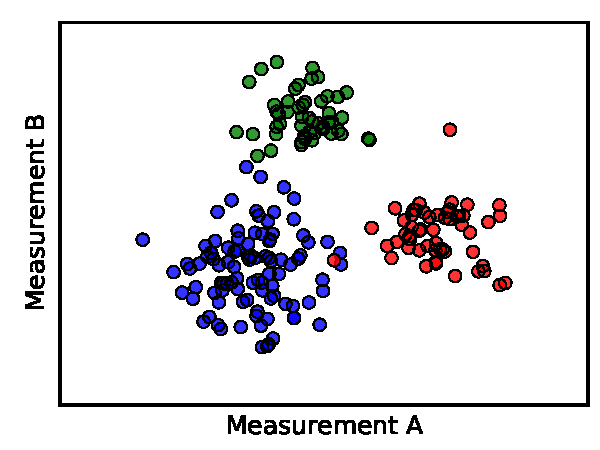
\includegraphics[width=0.4\textwidth]{ex3b}

\end{frame}

\section{K-means}

\begin{frame}{Clustering: the $K$-means algorithm}
  \begin{itemize}
    \item Assume $K$ \alert{clusters}, each characterized by a \alert{centroid}
    \item Start by randomly choosing $K$ data points as centroids
    \item Iteratively:
      \begin{itemize}
      \item \alert{Assign} each data point to the \alert{nearest} cluster
      \item \alert{Compute} new cluster center based on assigned data points
      \end{itemize}
  \end{itemize}
  \begin{center}
    \only<1>{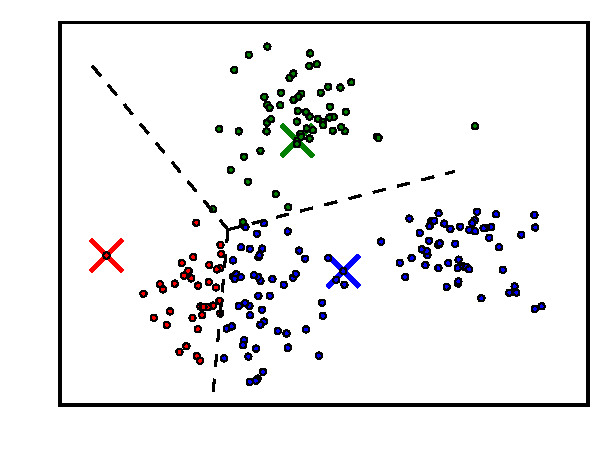
\includegraphics[width=0.7\textwidth]{kmeans-00}}%
    \only<2>{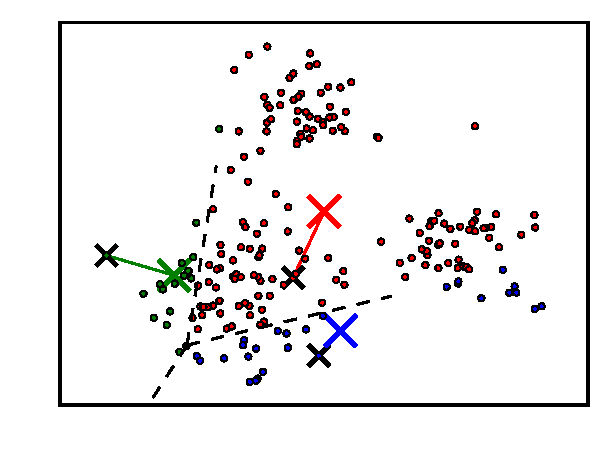
\includegraphics[width=0.7\textwidth]{kmeans-01}}%
    \only<3>{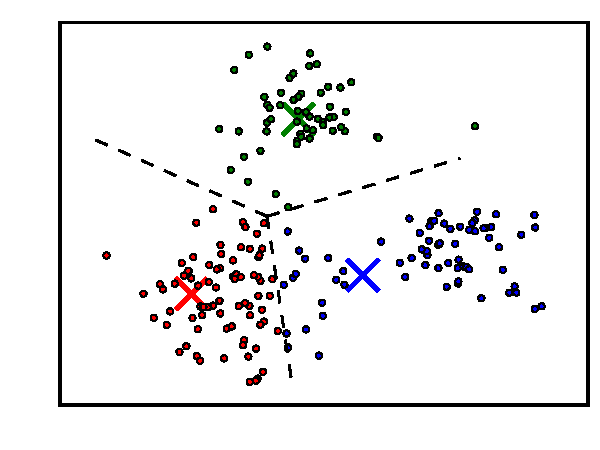
\includegraphics[width=0.7\textwidth]{kmeans-02}}%
    \only<4>{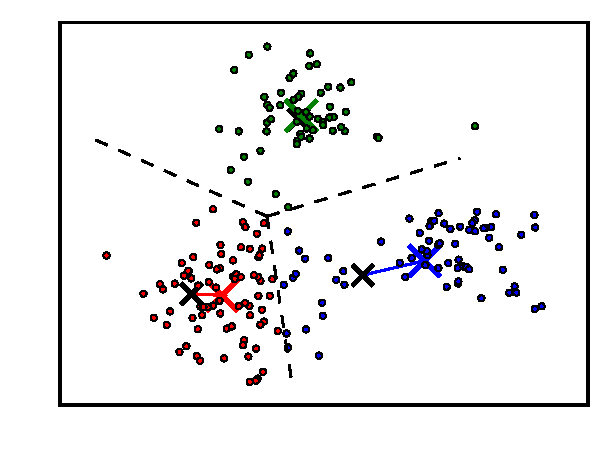
\includegraphics[width=0.7\textwidth]{kmeans-03}}%
    \only<5>{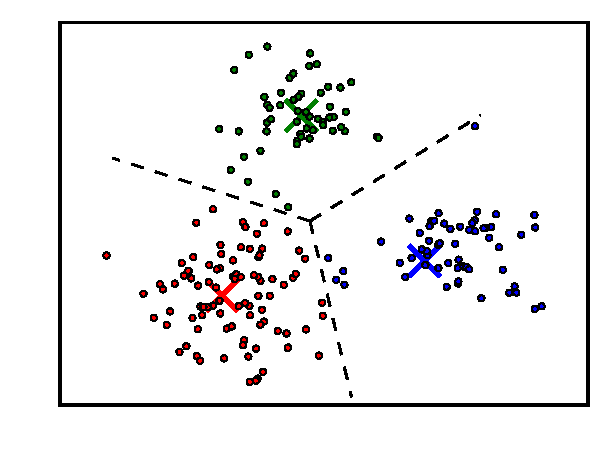
\includegraphics[width=0.7\textwidth]{kmeans-04}}%
    \only<6>{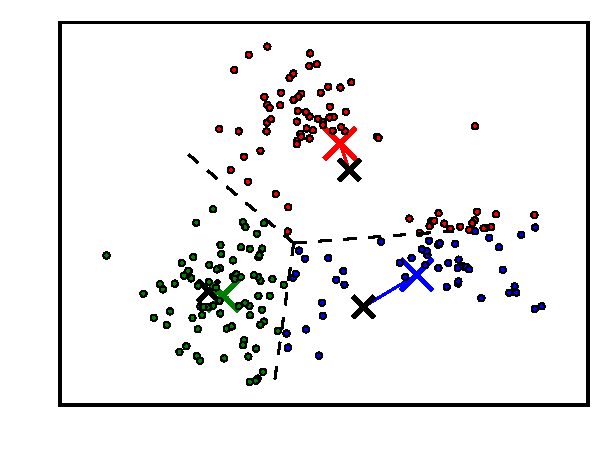
\includegraphics[width=0.7\textwidth]{kmeans-05}}%
    \only<7>{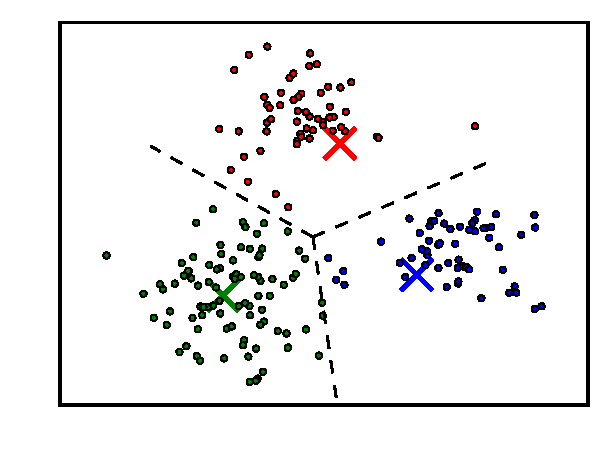
\includegraphics[width=0.7\textwidth]{kmeans-06}}%
    \only<8>{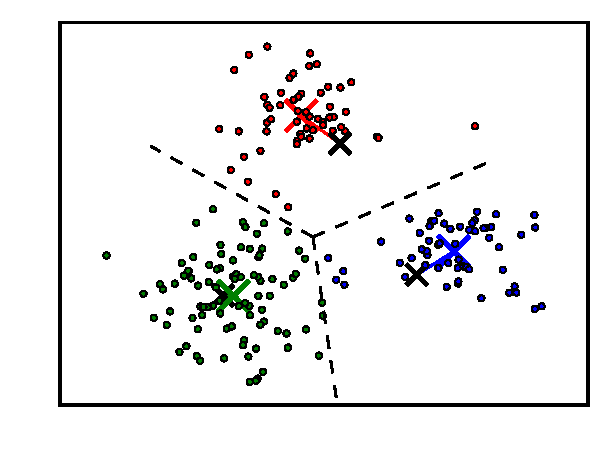
\includegraphics[width=0.7\textwidth]{kmeans-07}}%
    \only<9>{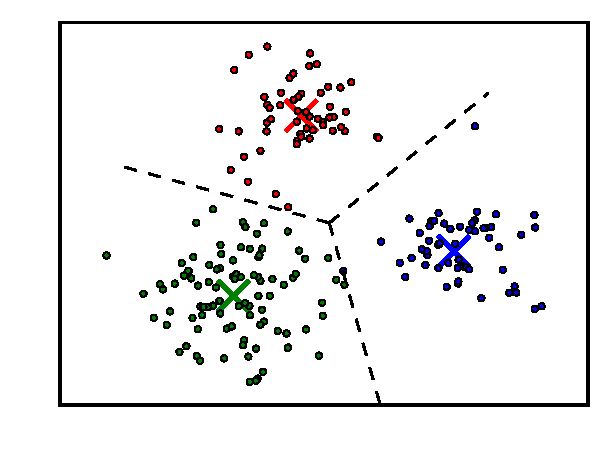
\includegraphics[width=0.7\textwidth]{kmeans-08}}%
    \only<10>{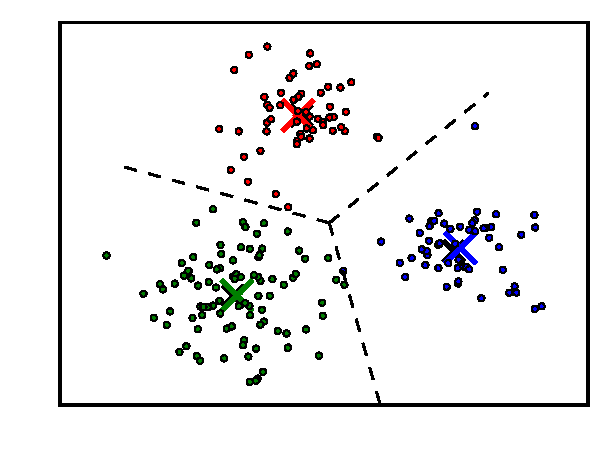
\includegraphics[width=0.7\textwidth]{kmeans-09}}%
    \only<11>{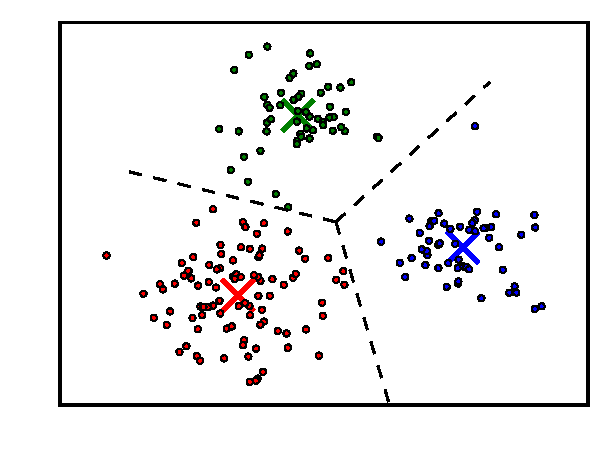
\includegraphics[width=0.7\textwidth]{kmeans-10}}%
  \end{center}
\end{frame}

\begin{frame}{Clustering: the $K$-means algorithm}
  \movie[showcontrols,once]{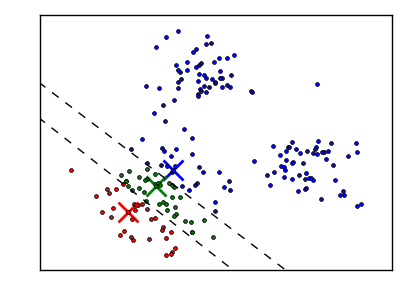
\includegraphics[width=\textwidth]{kmeans2-00}}{kmeans2.mov}
\end{frame}

% \begin{frame}{Breaking $K$-means}
%   Clusters are defined by \alert{centroids alone} $\longrightarrow$
%   Clusters split by hyper-planes
%   \begin{center}
%     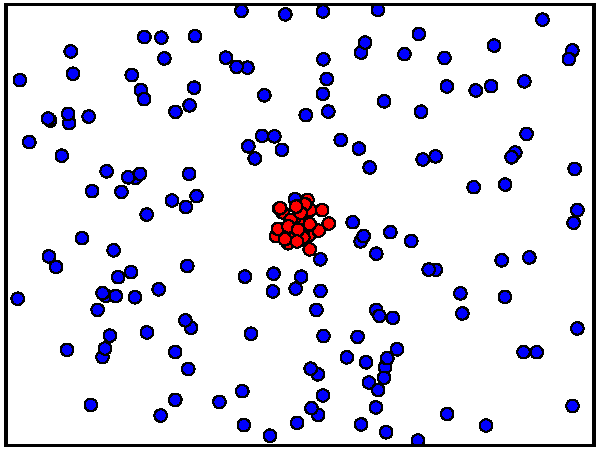
\includegraphics[width=0.49\textwidth]{break1-12}
%     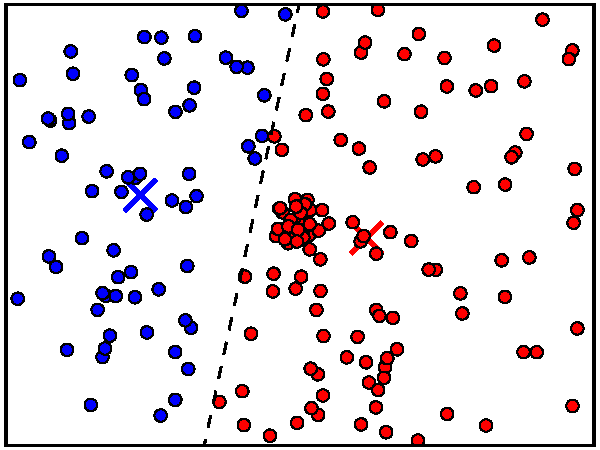
\includegraphics[width=0.49\textwidth]{break1-11}
%   \end{center}
% \end{frame}

\begin{frame}{Problems with $K$-means}
  Clusters are defined by \alert{centroids alone}
  \begin{itemize}
    \item clusters are separated by hyper-planes
    \item no covariances in the clusters
    \item no weights for clusters
    \item data points are hard-assigned to clusters
    \item noisy measurements not considered
    \item local optimization (multiple random initializations)
  \end{itemize}
  \begin{center}
    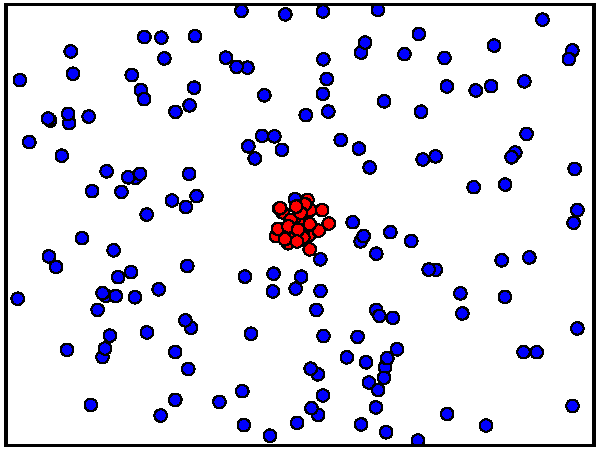
\includegraphics[width=0.49\textwidth]{break1-12}
    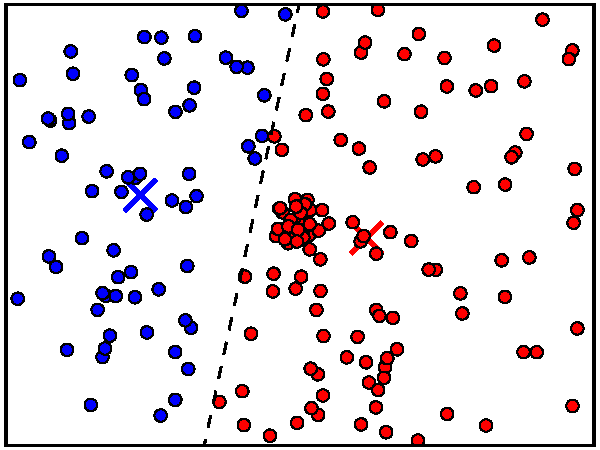
\includegraphics[width=0.49\textwidth]{break1-11}
  \end{center}
\end{frame}

\section{Mixture models}

\begin{frame}{Gaussian Mixture Models}
  \begin{itemize}
  \item Instead of finding just \alert{centroids}, we want to find
    \alert{weights} and Gaussians \alert{means} and
    \alert{covariances} of clusters
    %
  \item Can be optimized efficiently using the
    \alert{Expectation-Maximization} (EM) algorithm
  \end{itemize}

  \begin{center}
    \only<1>{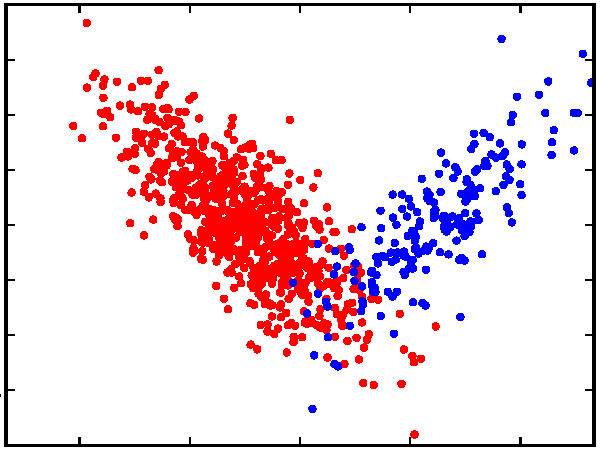
\includegraphics[width=0.66\textwidth]{gmm-00}}%
    \only<2>{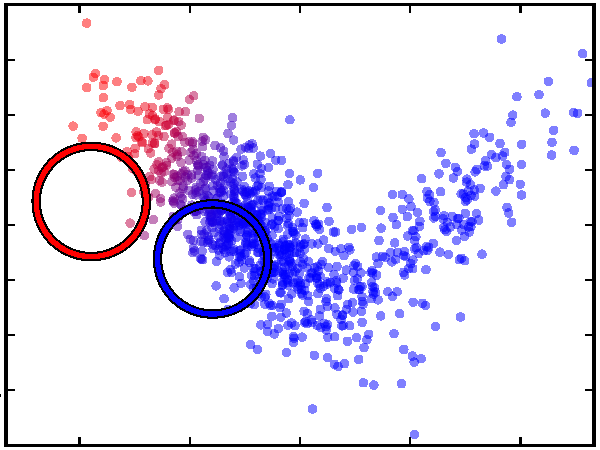
\includegraphics[width=0.66\textwidth]{gmm-01}}%
    \only<3>{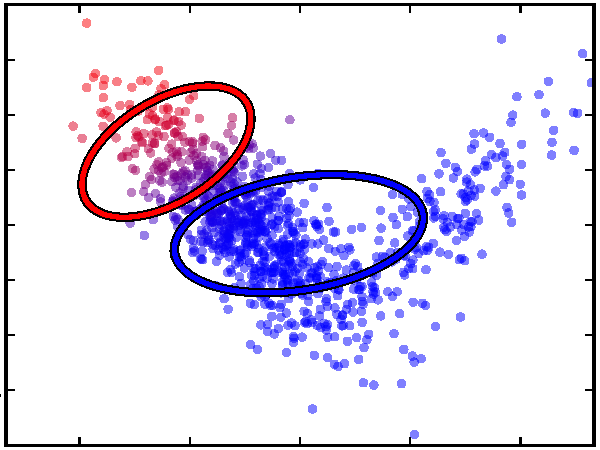
\includegraphics[width=0.66\textwidth]{gmm-02}}%
    \only<4>{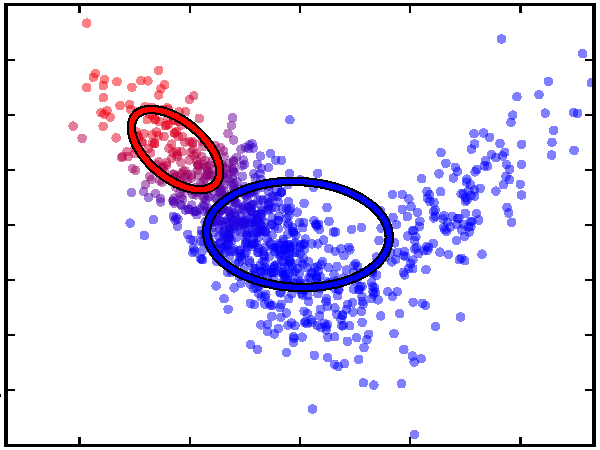
\includegraphics[width=0.66\textwidth]{gmm-03}}%
    \only<5>{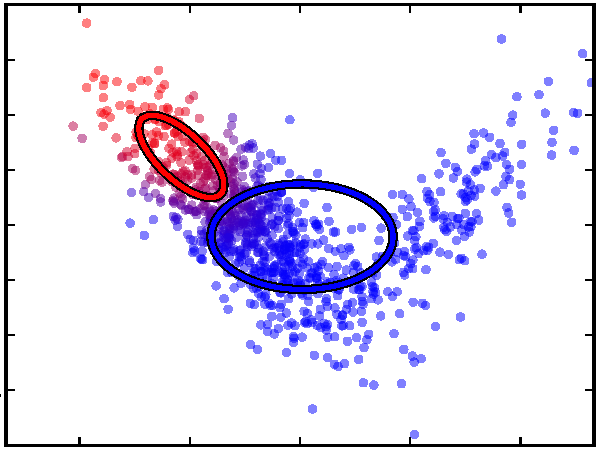
\includegraphics[width=0.66\textwidth]{gmm-04}}%
    \only<6>{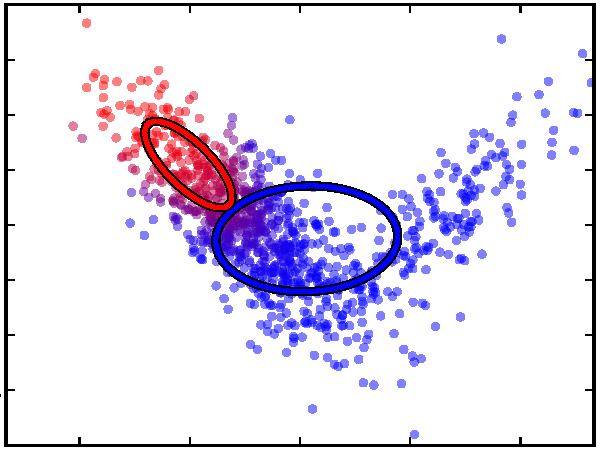
\includegraphics[width=0.66\textwidth]{gmm-05}}%
    \only<7>{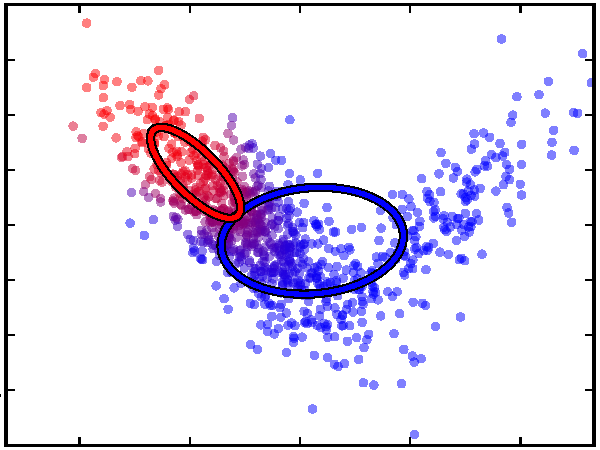
\includegraphics[width=0.66\textwidth]{gmm-06}}%
    \only<8>{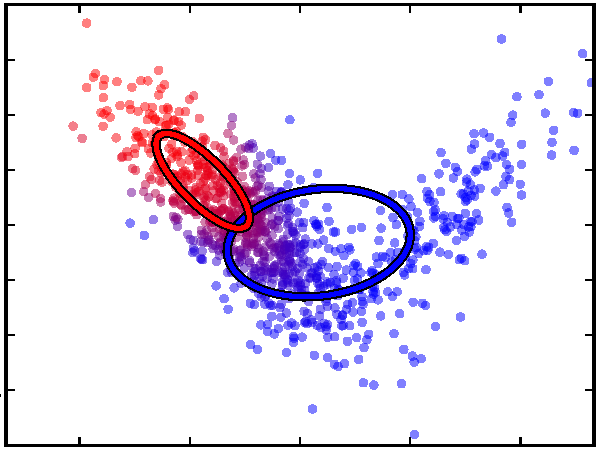
\includegraphics[width=0.66\textwidth]{gmm-07}}%
    \only<9>{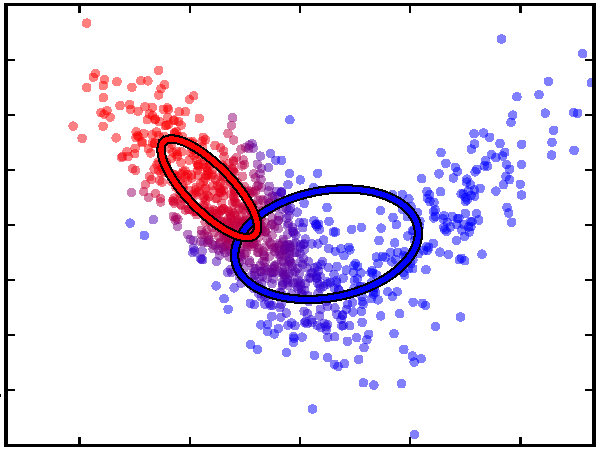
\includegraphics[width=0.66\textwidth]{gmm-08}}%
    \only<10>{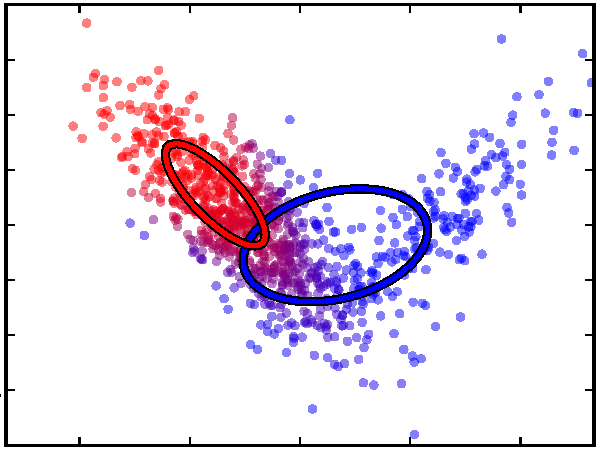
\includegraphics[width=0.66\textwidth]{gmm-09}}%
    \only<11>{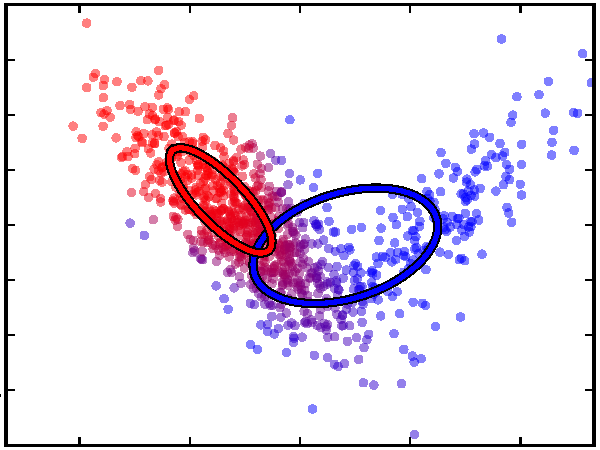
\includegraphics[width=0.66\textwidth]{gmm-10}}%
    \only<12>{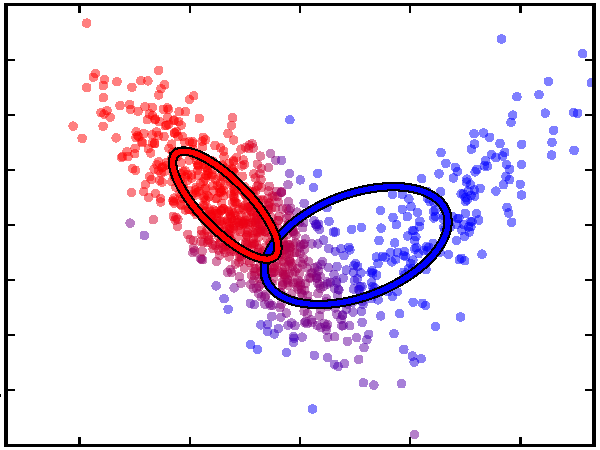
\includegraphics[width=0.66\textwidth]{gmm-11}}%
    \only<13>{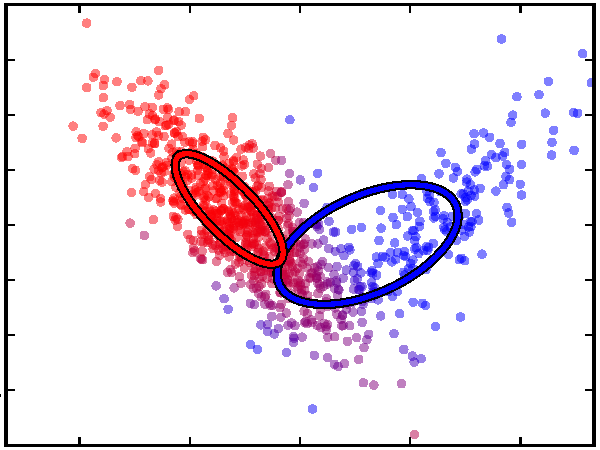
\includegraphics[width=0.66\textwidth]{gmm-12}}%
    \only<14>{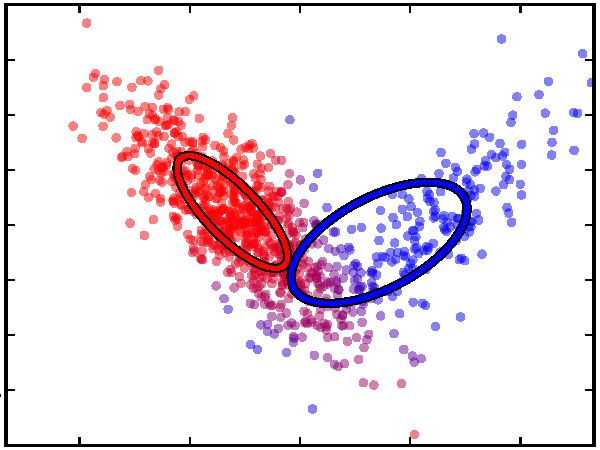
\includegraphics[width=0.66\textwidth]{gmm-13}}%
    \only<15>{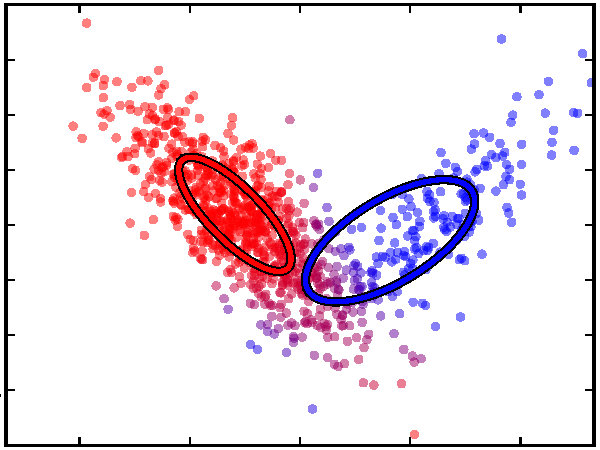
\includegraphics[width=0.66\textwidth]{gmm-14}}%
    \only<16>{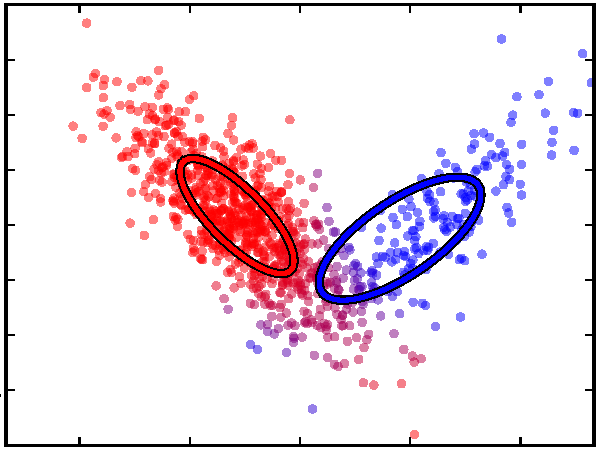
\includegraphics[width=0.66\textwidth]{gmm-15}}%
    \only<17>{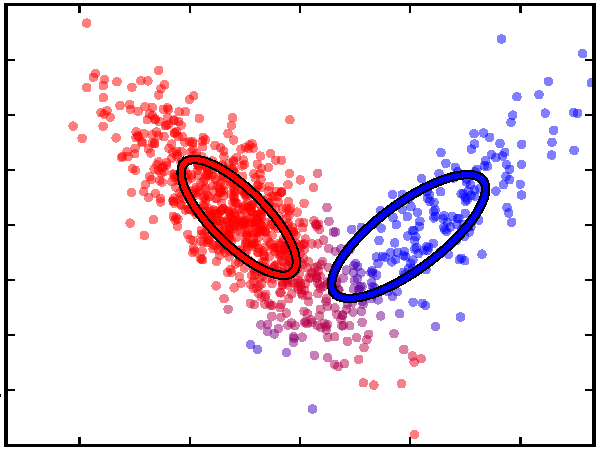
\includegraphics[width=0.66\textwidth]{gmm-16}}%
    \only<18>{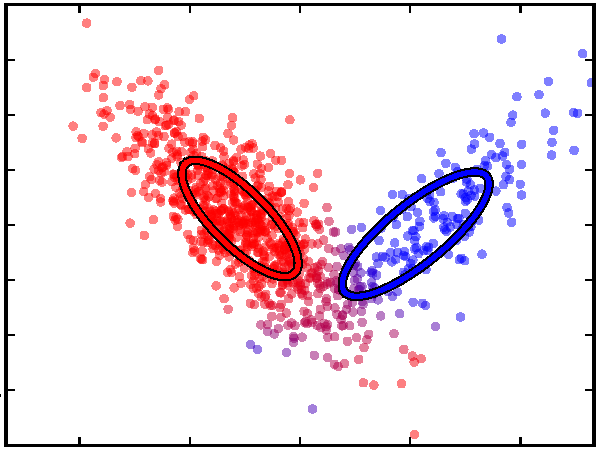
\includegraphics[width=0.66\textwidth]{gmm-17}}%
    \only<19>{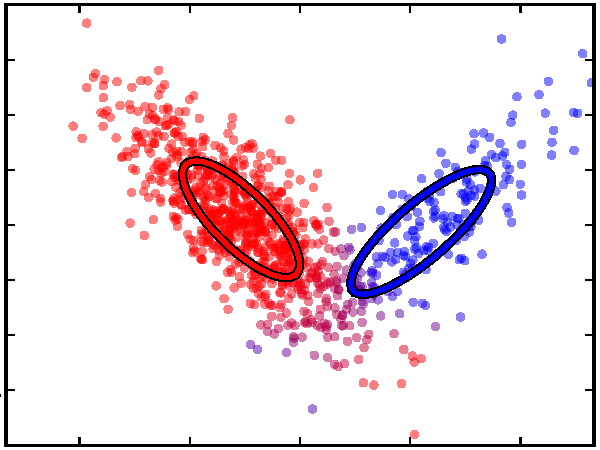
\includegraphics[width=0.66\textwidth]{gmm-18}}%
    \only<20>{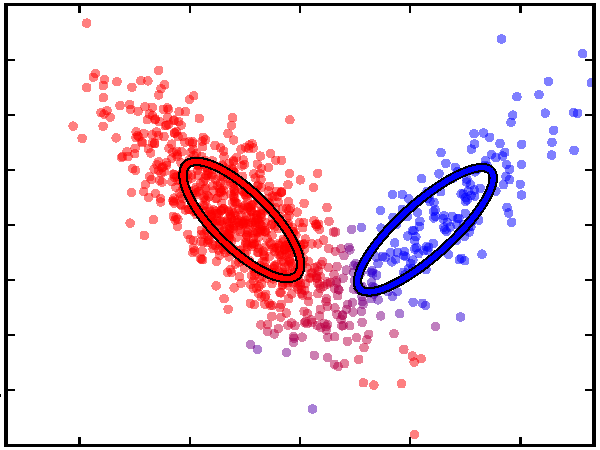
\includegraphics[width=0.66\textwidth]{gmm-19}}%
    \only<21>{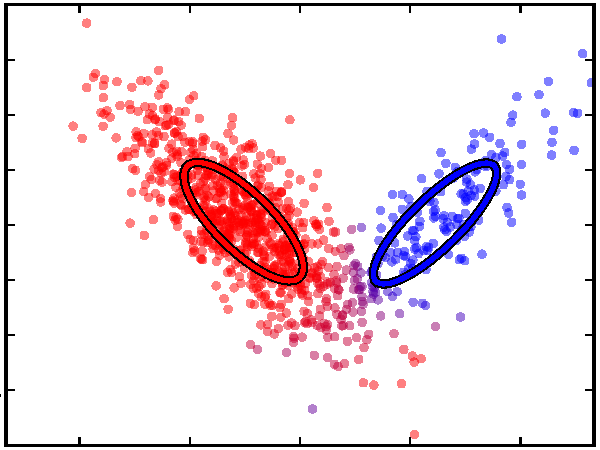
\includegraphics[width=0.66\textwidth]{gmm-24}}%
  \end{center}
\end{frame}

\begin{frame}{Gaussian Mixture Models / Expectation-Maximization}
  E-M proceeds by:
  \begin{itemize}
  \item \alert{E}: compute probability of drawing each \alert{data
    point} $i$ from each \alert{cluster} or \alert{component} $k$:
    \[
    z_{i,k} = a_k \, \mathcal{N}(x_i \,|\, \mu_k, \Sigma_k)
    \]
  where $a_k$ is the cluster \alert{weight}, and $\mu_k$,$\Sigma_k$
  are its mean and covariance.
    %
  \item \alert{M}: compute new component weights and parameters,
    weighting by \emph{relative} component-weights
  \end{itemize}
\end{frame}

\begin{frame}{Gaussian Mixture Models / Expectation-Maximization}
  \begin{itemize}
    \item E-M ``update equations'' (M step) for Gaussian mixtures:
      \begin{align}
        z'_{i,k} &= \frac{z_{i,k}}{\sum_k z_{i,k}} \\
        a'_k &= \sum_k z'_{i,k} \\
        \mu'_{i,k} &= \frac{1}{a'_k} \, z'_{i,k} x_i \\
        \Sigma'_{i,k} &= \frac{1}{a'_k} \, z'_{i,k} (x_i - \mu_k) (x_i - \mu_k)^T
      \end{align}
  \end{itemize}
\end{frame}


\begin{frame}{Mixture Models / Foreground-Background Models}
  \begin{itemize}
    \item Often, \alert{junk} or \alert{interlopers} can get into your
      sample (of galaxies, stars, etc)
    \item If not dealt with, can strongly skew results (outliers)
    \item \alert{Model} the objects you don't care about (background)
      \alert{as well as} the ones you do care about (foreground)
    \item Background model can be a regular Gaussian component, or a
      flat (uniform) probability distribution
  \end{itemize}
  \begin{center}
    \only<1>{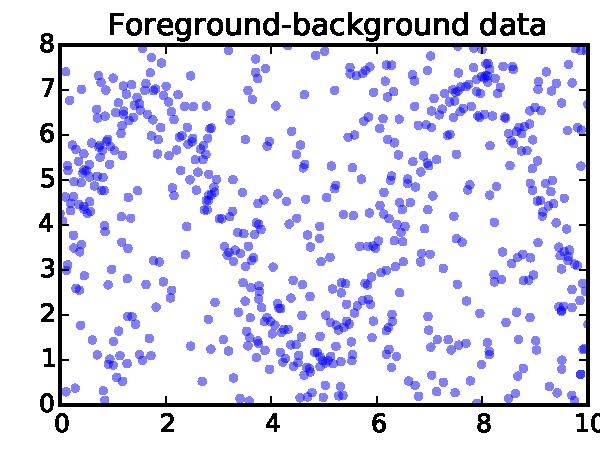
\includegraphics[width=0.5\textwidth]{fgbg-0}}%
    \only<2>{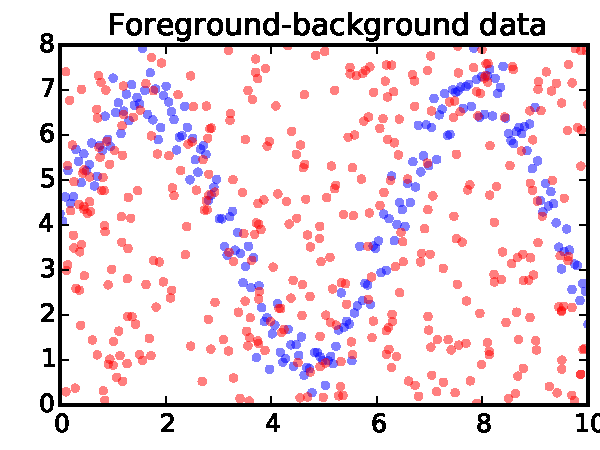
\includegraphics[width=0.5\textwidth]{fgbg-1}}%
    \only<3>{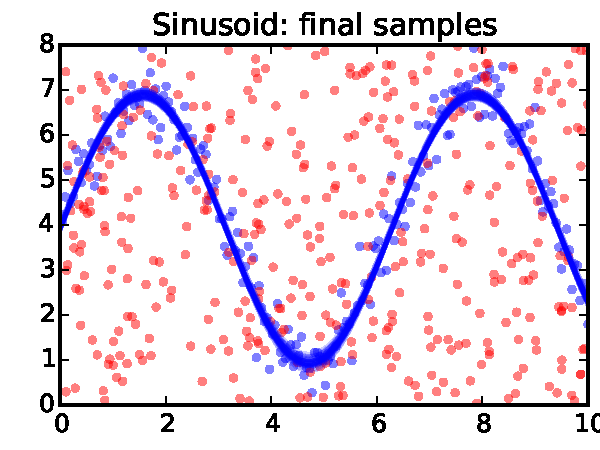
\includegraphics[width=0.5\textwidth]{fgbg-2}}%
  \end{center}
\end{frame}

% \begin{frame}{Problems with Gaussian Mixture Models}
%   \begin{itemize}
%   \item Choosing the number of components
%   \item Measurement noise not considered
%   \item Local optimization
%   \end{itemize}
% \end{frame}


% \begin{frame}{Summary -- Unsupervised Learning}
%   \begin{itemize}
%     \item I haven't talked about \alert{Dimensionality Reduction}
%   \end{itemize}
% \end{frame}


\end{document}

